% \documentclass[letterpaper,12pt]{article}
\documentclass[a4paper,10pt]{article}
\usepackage[total={18cm,20cm}, top=1.5cm, left=1.5cm]{geometry}
\usepackage[spanish]{babel}
\usepackage[utf8]{inputenc}
% \usepackage[latin1]{inputenc}
\usepackage[T1]{fontenc}
\usepackage{graphicx}
\usepackage{subfigure}
\usepackage{fancyhdr}
\usepackage{setspace}
\usepackage{hyperref}

\renewcommand{\baselinestretch}{1.5}
\pagestyle{fancy}
\rhead{
\includegraphics[width = .065\textwidth]{imagenes/LogoBase.png}}
\lhead{\textit{Social Data Mining \& statistics}}

% \fancyfoot[R]{\includegraphics[width=5mm]{./imagenes/logo.png}}

\title{Análisis de la interacción de los posteos de SEAT, en base al número de posteos
realizados}
\author{Social Data Mining \& Statistics \\
        Base10}
% \subtitle{LatReach}
\date{}


\begin{document}
\maketitle

% \begin{abstract}
% \end{abstract}

\section{Introducción}
Hasta el mes de Junio de 2016, la población humana era de 7,340,156,492 personas, 
de toda esa población el 50.1 \% (3,675,824,813) utilizaban internet
(Internet World Stats, 2016).\\
De la gran cantidad de páginas que existen en Internet, Facebook es una de las 
más utilizadas, con un promedio de 1040 millones de personas conectadas diariamente 
a este sitio web (Facebook statistics, 2016).\\
Facebook es una red social, al igual que otros sitios web como Twitter o Instagram,
no obstante, Facebook lidera en el número de usuarios (Smarthinsights, 2016).
La popularidad y por ende el uso de las redes sociales obedece a que los 
seres humanos son altamente dependientes del soporte social de otros seres
de su misma especie. Por lo tanto, las redes sociales satisfacen dos necesidades
primordiales de los seres humanos: Necesidad de autorepresentación y la necesidad
de pertenencia a un grupo (Nadkarni y Hofmann, 2012).\\
Más allá del impacto social y de comportamiento que pueda tener Facebook,
esta red social puede ser utilizada para diversos fines, que van desde la investigación 
y finalizando con el mercadeo (marketing) (Wilson et al, 2012).
Para el caso del mercadeo, Facebook es uno de los sitios en los cuales
las personas pasan una gran cantidad de su tiempo, por lo tanto podría considerarse
un gran canal para dar anuncios de diversas empresas (Roshnee y Fowdar, 2013).
En otros aspectos, Facebook puede ayudar a comprender el 
comportamiento de sus potenciales consumidores .
Por otro lado es posible realizar estrategias específicas para los potenciales
consumidores o seguidores de las redes sociales de alguna marca en particular (Casteleyn et al, 2009).\\
Sin embargo, la forma de interacción entre empresa y consumidor, cambia
con el tiempo, debido a diversos factores, uno de ellos es el cambio constante
del algoritmo de Facebook encargado de regular la sección de noticias de cada usuario (\textit{EdgeRank}).
De esta manera, las empresas deben cambiar regularmente la manera en como interactúan
con sus seguidores.
\\ [5cm]
La forma más común de interactuar con los seguidores de cierta empresa es realizar
posteos(publicar imágenes, texto, video) en los perfiles públicos de las mismas empresas.
Estos posteos son la base para poder obtener las diversas métricas que las empresas
necesitan para poder comprender el comportamiento  de sus usuarios o potenciales
compradores.\\
Postear demasiado o poco, puede resultar arriesgado, puesto que en promedio 
cada usuario de Facebook tiene 1500 publicaciones nuevas
diarias en su muro, ya sea de sus amigos, seguidores o sitios que el usuario sigue (Facebook business, 2013).
En general, del gran número de publicaciones que un usuario tiene en su muro, solo puede ver un pequeño porcentaje de estas.

De manera general, el número de posteos realizados por determinada empresa va de la mano
con el número de usuarios que siguen a la misma. Patel (2012) propuso que si se tiene al menos
10,000 seguidores lo ideal sería postear al menos dos veces al día y eso te garantizaba una 
buena suma de ``clicks''  e interacciones.

No obstante con el cambio constante del algoritmo \textit{EdgeRank}, actualmente es
muy dificil garantizar una gran interacción.
Muchos sitios recomiendan que para tener una gran interacción, se necesitan de al menos
dos características importantes para cada posteo: Un gran incentivo (foto, video, gif) 
y una corta descripción que incite a realizar una acción (``click'' p.ej).\\
Para nuestro caso en particular, SEAT  de México se esfuerza en realizar cuatro posteos
diarios. Contando con 1 millon 600 mil seguidores a la fecha.
Para mejorar la calidad de los posteos y obtener la misma o una mayor cantidad de métricas
positivas en la cuenta de Facebook de SEAT.
Se propone un experimento que consiste en bajar el número de posteos a tres por día para
comprender la dinámica de las interacciones para la cuenta de SEAT.
Para realizar dicho experimento, se planea comparar las interacciones resultantes 
producidas por los tres posteos diarios con las interacciones de una semana con cuatro posteos.



\section{Objetivo general}
Determinar los efectos en las interacciones al realizar tres posteos diarios en la 
cuenta de Facebook de SEAT.


\section{Objetivos particulares}
  \begin{itemize}
   \item[$*$] Conocer el enganche (``engagement'') y alcance producto de la disminución de las publicaciones.
   \item[$*$] Conocer la cantidad de comentarios, reacciones, número de veces que se comparte una publicación al disminuir las publicaciones.
   \item[$*$] Comparar el número interacciones de una semana con tres posteos al día contra otra de cuatro posteos diarios.
  \end{itemize}


\section{Metodología}
El experimento consiste en un periodo de dos semanas (14 días).
La primera semana de experimento consiste en realizar tres posteos al día (21 posteos a la semana).
24 horas después de cada posteo, se medirán el número de interacciones para dicho posteo.
Esto con el objetivo de tener datos homogeneizados para cada posteo.
Para el caso de la segunda semana, la estrategia será la misma, con la única diferencia de que serán cuatro posteos
al día (28 posteos a la semana) (Figura 1).
\begin{figure}[h]
  \begin{center}
   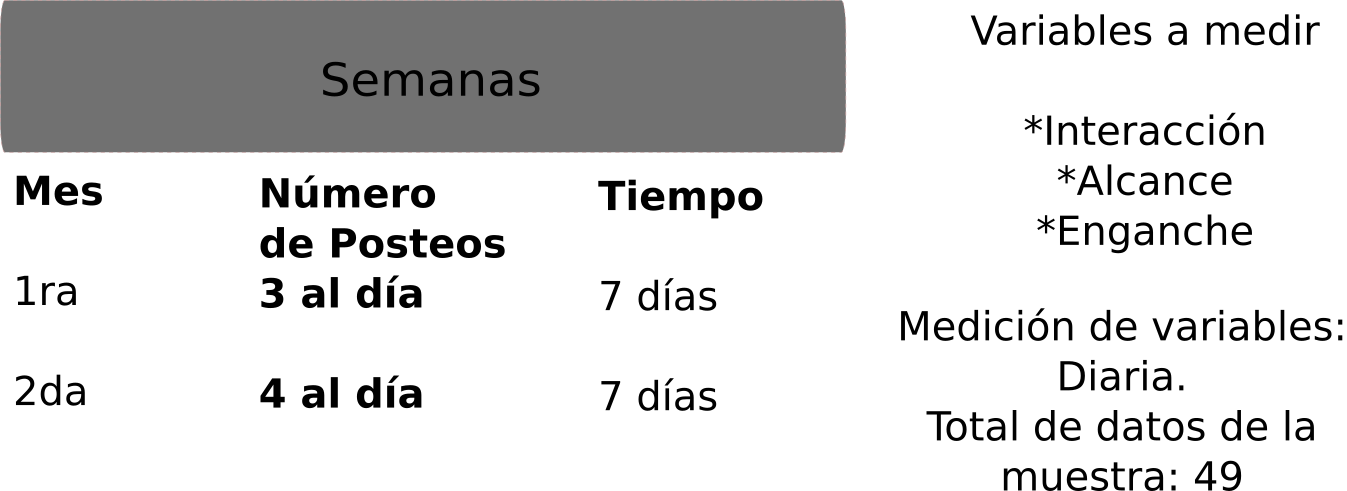
\includegraphics[width=.75\textwidth]{imagenes/dibujoExperimentoNuevo.png}
   \caption{Diseño experimental}
  \end{center}

 
\end{figure}



\section{Análisis estadísticos}
El número de interacciones serán analizados en conjunto y por tipo de interacción mediante análisis de varianza (ANOVA) bifactoriales (Zar, 2010) 
o modelos lineales generalizados (GLM), el tipo de análisis a utilizar dependerá de la distribución de error de los datos, 
que servirá de base para tener en cuenta el modelo a utilizar.

\begin{thebibliography}{10}
  \bibitem{1} Casteleyn J; Mottart A; Rutten K. (2009). How to use Facebook in you market research. International Journal of Market Research. 51(4) 439-447.
  \bibitem{2} Facebook. (2016). \textit{ Statistics of  Facebook}, Palo  Alto,  CA:  Facebook. Tomado de: http://ltam.newsroom.fb.com/company-info/
  \bibitem{3} Facebook business. (2013). Tomado de: https://www.facebook.com/business/news/News-Feed-FYI-A-Window-Into-News-Feed
  \bibitem{4} Internet World Stats. (2016). Tomado de: http://www.internetworldstats.com/stats.htm
  \bibitem{5} Nadkarni A; Hofmann S. (2012). Why Do People Use Facebook . Personality and Individual Differences. 52(2012) 243-249
  \bibitem{6} Patel N. (2012). How Frequently You Should Post on Social Media According to the Pros. Forbes. Tomado de: http://www.forbes.com/sites/neilpatel/2016/09/12/how-frequently-you-should-post-on-social-media-according-to-the-pros/#3d7172ca36d5
  \bibitem{7} Roshnee R; Fowdar S. (2013). The implications of Facebook Marketing for Organizations. Contemporay Management Research. 9 (1) 73-84. doi:10.7903/cmr.9710
  \bibitem{8} Smarth Insights. (2016). Global social media research summary 2016. Tomado de: http://www.smartinsights.com/social-media-marketing/social-media-strategy/new-global-social-media-research/
  \bibitem{9} Wilson R; Gosling S; Graham L. (2012). A review of Facebook research in the social sciences. Perspectives on Psychological Science 7 (3) 203-220
  \bibitem{10} Zar J. (2010). Biostatistical Analysis. Pearson Prentice Hall. New Jersey. ISBN-10: 0-13-100846-3
\end{thebibliography}

\end{document}
